\documentclass[11pt]{article}
\usepackage[margin=1in]{geometry}
\usepackage{authblk}
\usepackage{amsmath,amssymb}
\usepackage{graphicx}
\usepackage{caption}
\usepackage{subcaption}
\usepackage{float}
\usepackage{placeins}
\usepackage{array}
\usepackage{tabularx}
\usepackage[numbers,sort&compress]{natbib}
\usepackage{hyperref}
\hypersetup{colorlinks=true,linkcolor=black,citecolor=black,urlcolor=black}

\graphicspath{{figures_supp/}{figures/}}

\newcolumntype{Y}{>{\raggedright\arraybackslash}X}
\newcolumntype{C}{>{\centering\arraybackslash}X}
\captionsetup[subfigure]{labelformat=empty,skip=0pt}

% Supplementary numbering (S1, S2, ...; Figure S1; Table S1)
\renewcommand{\thesection}{S\arabic{section}}
\renewcommand{\thesubsection}{S\arabic{section}.\arabic{subsection}}
\renewcommand{\thesubsubsection}{S\arabic{section}.\arabic{subsection}.\arabic{subsubsection}}
\renewcommand{\thefigure}{S\arabic{figure}}
\renewcommand{\thetable}{S\arabic{table}}

\title{Supplementary Materials for:\\Phase Transitions in Collective Emotion: A Theoretical Framework Motivated by Media Dynamics During the COVID-19 Pandemic}
\author[1]{Author A (TBD)}
\affil[1]{Affiliation TBD}
\date{}

\begin{document}
\maketitle

\renewcommand{\contentsname}{Supplementary Contents}
\setcounter{tocdepth}{2}
\tableofcontents
\clearpage
\FloatBarrier

\section*{Guide to this Supplementary Materials}
\addcontentsline{toc}{section}{Guide to this Supplementary Materials}
This document provides supporting details that cannot be fully developed in the main text due to space constraints. It is organized to mirror the main-text workflow and results: S1--S2 extend the \emph{Materials and Methods}, and S3--S6 provide additional diagnostics for the \emph{Results}. The main text cites these materials as ``Supplementary Materials S\#'' and ``Supplementary Fig.~S\#''.

\noindent\textbf{Contents overview.}
\begin{itemize}
  \item \textbf{Supplementary Methods}
  \begin{itemize}
    \item \textbf{S1} LLM annotation protocol and validation.
    \item \textbf{S2} Mean-field derivations for the critical point and Ginzburg--Landau form.
  \end{itemize}
  \item \textbf{Supplementary Results}
  \begin{itemize}
    \item \textbf{S3} Additional theory and network-validation diagnostics.
    \item \textbf{S4} Additional critical-slowing-down diagnostics.
    \item \textbf{S5} Additional parameter-landscape analyses.
    \item \textbf{S6} Additional empirical analyses and robustness checks.
  \end{itemize}
\end{itemize}
\FloatBarrier

\section*{Supplementary Methods}
\addcontentsline{toc}{section}{Supplementary Methods}
\noindent Sections S1--S2 provide additional methodological details for the empirical annotation pipeline and the mean-field derivations.
\FloatBarrier

% -------------------------
% S1: LLM annotation protocol
% -------------------------
\section{LLM annotation protocol}
\label{supp:s1-llm}

This note documents the LLM-based annotation pipeline used to label Weibo posts for emotional arousal and risk content.

\subsection{Model and infrastructure}

\begin{itemize}
  \item Model: \texttt{Qwen/Qwen3-8B}.
  \item Serving: vLLM via an OpenAI-compatible Chat Completions API.
  \item Client: \texttt{openai} Python client, enforcing a single JSON object output using \texttt{response\_format=\{"type":"json\_object"\}}.
\end{itemize}

\subsection{Inference settings}

\begin{itemize}
  \item Temperature: 0.1
  \item Max tokens: 512
\end{itemize}

\subsection{Annotation tasks}

Each post is labeled along two dimensions:
\begin{itemize}
  \item Emotional arousal (\texttt{emotion\_class}): \texttt{H} (high), \texttt{M} (medium/neutral), \texttt{L} (low).
  \item Risk content (\texttt{risk\_class}): \texttt{risk} vs.\ \texttt{norisk}.
\end{itemize}

\subsection{Prompt template and output schema}

We use a structured prompt that defines label criteria and requires the model to output a single JSON object (no additional text). The implementation is in \texttt{src/empirical/llm\_annotator.py} and is invoked by \texttt{scripts/run\_new\_annotation.py}.

\subsubsection{System prompt (English translation for readability)}

\begin{verbatim}
You are an expert in social media content analysis. Your task is to label each Weibo post
along two dimensions: emotional arousal and risk content. Output exactly one JSON object
and nothing else (no chain-of-thought, no markdown).

Emotion arousal (emotion_class):
- H (high arousal): strong emotions (anger, fear/panic, sarcasm, insults, highly emotional accusations).
- M (medium/neutral): factual or calm discussion, neutral reposts/comments, supportive messages, explanations.
- L (low arousal): negative but not intense emotions (anxiety, worry, confusion, helplessness, sadness).

Risk content (risk_class):
Core rule: does the post convey that COVID-19/long COVID has negative health impacts?
- risk: describes symptoms/health changes, emphasizes severity/long-term/irreversibility, warns about risks,
        reports cases/studies of sequelae, questions "no sequelae" claims, or raises risk-focused questions.
- norisk: emphasizes recovery/controllability, reassuring official explanations, criticizes fear-mongering,
          success stories stressing recovery, or content unrelated to long-COVID health risks.

Edge cases:
- Very short/hashtag-only posts with no substance: default to M + norisk, confidence 0.5.
- Light tone does not imply norisk: joking symptom descriptions are still risk.

Output JSON format (and only this):
{"emotion_class": "H"|"M"|"L",
 "emotion_confidence": 0.0-1.0,
 "risk_class": "risk"|"norisk",
 "risk_confidence": 0.0-1.0,
 "reasoning": "brief justification"}
\end{verbatim}

\subsubsection{User prompt}

\begin{verbatim}
Please analyze the following Weibo post:

---
{text}
---

Return the classification result in JSON format as specified.
\end{verbatim}

\subsubsection{Output fields}

The model must output a single JSON object with the following fields:
\begin{itemize}
  \item \texttt{emotion\_class}: one of \texttt{H}, \texttt{M}, \texttt{L}.
  \item \texttt{emotion\_confidence}: a float in $[0,1]$.
  \item \texttt{risk\_class}: one of \texttt{risk}, \texttt{norisk}.
  \item \texttt{risk\_confidence}: a float in $[0,1]$.
  \item \texttt{reasoning}: a short justification string.
\end{itemize}

\subsection{Validation}

We compared LLM-assigned labels to manual ratings on a manually rated subset ($n=3{,}000$). Overall exact-match agreement (accuracy) between LLM and human labels was 83\%.

% -------------------------
% S2: Mean-field derivations
% -------------------------
\section{Mean-field derivations}
\label{supp:s2-mean-field}

This note provides the derivations omitted from the main text for the mean-field critical point and the Ginzburg--Landau form.

\subsection{Mean-field update and collective response}

Under well-mixed assumptions, each update samples $k$ independent risk signals from the environment, each labeled ``risk'' with probability $p_{\text{env}}$. Let $S\sim\text{Binomial}(k,p_{\text{env}})$ and $\hat{p}=S/k$ be the perceived risk fraction. Given thresholds $\theta<\phi$, an updated individual moves to $H$ if $\hat{p}\ge \phi$, to $L$ if $\hat{p}\le \theta$, and otherwise remains in $M$. Therefore,
\begin{align}
P_H(p_{\text{env}}) &= \Pr(\hat{p}\ge \phi)=\sum_{s=\lceil k\phi\rceil}^{k}\binom{k}{s}p_{\text{env}}^{\,s}(1-p_{\text{env}})^{k-s},\\
P_L(p_{\text{env}}) &= \Pr(\hat{p}\le \theta)=\sum_{s=0}^{\lfloor k\theta\rfloor}\binom{k}{s}p_{\text{env}}^{\,s}(1-p_{\text{env}})^{k-s}.
\end{align}
The expected polarization direction after an update is the difference between high- and low-arousal outcomes,
\begin{equation}
\mathcal{S}(p_{\text{env}})=P_H(p_{\text{env}})-P_L(p_{\text{env}}).
\end{equation}
With asynchronous updates and a continuous-time approximation, the mean-field dynamics take the form
\begin{equation}
\frac{dq}{dt}=-q+\mathcal{S}(p_{\text{env}}),
\end{equation}
which is the mean-field form used in the main text.

\subsection{Linear stability and analytic critical point}

In the symmetric validation regime,
\begin{equation}
p^{\text{main}}(q)=\frac{1-q}{2},\qquad p^{\text{we}}(q)=\frac{1+q}{2}.
\end{equation}
The environmental risk is the weighted average of the two channels,
\begin{equation}
p_{\text{env}}(q;r)=\frac{(1-r)n_m p^{\text{main}}(q)+r n_w p^{\text{we}}(q)}{(1-r)n_m+r n_w},
\end{equation}
where $n_m$ and $n_w$ are baseline channel strengths and $r\in[0,1]$ controls their relative weight. Expanding around $q=0$ yields
\begin{equation}
p_{\text{env}}(q;r)=\frac{1}{2}+\Gamma(r)\,q+O(q^3),
\end{equation}
where the feedback gradient is
\begin{equation}
\Gamma(r)=\left.\frac{\partial p_{\text{env}}}{\partial q}\right|_{q=0}
=\frac{r n_w-(1-r)n_m}{2\left((1-r)n_m+r n_w\right)}.
\end{equation}
Next, expand the collective response around neutrality $p=1/2$:
\begin{equation}
\mathcal{S}(p)=\mathcal{S}(1/2)+\chi\left(p-\frac{1}{2}\right)+O\!\left(\left(p-\frac{1}{2}\right)^3\right),\qquad
\chi=\left.\frac{d\mathcal{S}}{dp}\right|_{p=1/2}.
\end{equation}
Under symmetry, $\mathcal{S}(1/2)=0$, so substituting $p_{\text{env}}(q;r)$ into the mean-field dynamics gives, to leading order,
\begin{equation}
\frac{dq}{dt}=(-1+\chi\Gamma)\,q+O(q^3).
\end{equation}
Therefore the neutral fixed point $q=0$ loses stability when the linear restoring coefficient changes sign:
\begin{equation}
\chi\Gamma(r_c)=1.
\end{equation}
Solving for $r$ yields the closed-form critical point reported in the main text:
\begin{equation}
r_c=\frac{n_m(\chi+2)}{n_m(\chi+2)+n_w(\chi-2)}.
\end{equation}
When $\chi\le 2$, the denominator does not admit a critical point in $[0,1]$, consistent with the absence of a transition for weak psychological sensitivity.

\subsection{Ginzburg--Landau form and noise term}

Keeping the next nonlinearity in the expansion yields a cubic term. Writing
\begin{equation}
\mathcal{S}(p)=\chi\left(p-\frac{1}{2}\right)+\frac{\mathcal{S}^{(3)}(1/2)}{6}\left(p-\frac{1}{2}\right)^3+O\!\left(\left(p-\frac{1}{2}\right)^5\right),
\end{equation}
and using $p_{\text{env}}-1/2\approx \Gamma q$, we obtain
\begin{equation}
\frac{dq}{dt}=(-1+\chi\Gamma)\,q+\frac{\mathcal{S}^{(3)}(1/2)}{6}\Gamma^3 q^3+\eta(t)+\cdots
=-\alpha q-u q^3+\eta(t)+\cdots,
\end{equation}
where $\alpha=1-\chi\Gamma$ and $u=-\mathcal{S}^{(3)}(1/2)\Gamma^3/6$. For the parameter ranges considered, $u>0$, so the dynamics can be written in the effective-potential form
\begin{equation}
\frac{dq}{dt}=-\frac{\partial V_{\text{eff}}(q)}{\partial q}+\eta(t),\qquad
V_{\text{eff}}(q)=\frac{1}{2}\alpha q^2+\frac{u}{4}q^4,
\end{equation}
which gives a pitchfork bifurcation when $\alpha$ changes sign.

The noise term $\eta(t)$ represents stochastic fluctuations induced by finite population size and discrete updates. In the large-$N$ limit, these fluctuations can be approximated as Gaussian white noise with an amplitude that scales as $1/\sqrt{N}$, implying a variance scaling as $1/N$.
\FloatBarrier

\section*{Supplementary Results}
\addcontentsline{toc}{section}{Supplementary Results}
\noindent Sections S3--S6 provide additional figures and robustness checks that support the main-text results, organized in the same order as the Results section.
\FloatBarrier

% -------------------------
% S3: Additional theory and network-validation diagnostics
% -------------------------
\section{Additional theory and network-validation diagnostics}
\label{supp:s3-theory-network}

This note provides robustness checks supporting the theoretical and network-validation results in the main text. The additional analyses below clarify the order-parameter conventions used to visualize the transition, validate that the activity variable carries independent dynamical information under realistic asymmetry, and motivate the finite-size estimator used to locate the transition in sparse networks.

\subsection{Order parameter under symmetric branch selection}
In the symmetric validation regime, different realizations can select either the $+q^\ast$ or $-q^\ast$ branch with approximately equal probability. As a result, the signed mean $\langle Q\rangle$ cancels even when the bifurcation exists, while $|Q|$ (or sign-aligned $Q$) recovers the transition curve used in the main text.

\begin{figure}[H]
  \centering
  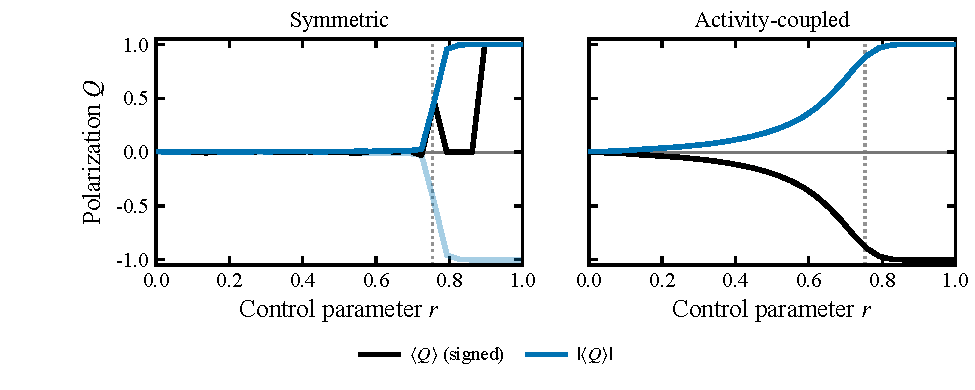
\includegraphics[width=0.92\linewidth]{s2_signed_vs_abs_q.pdf}
  \caption{Signed vs.\ magnitude order parameters under symmetric branch selection. In the symmetric regime, independent realizations select either the $+q^\ast$ or $-q^\ast$ branch with (approximately) equal probability, so the signed mean $\langle Q\rangle$ cancels even when a bifurcation exists. Using $|Q|$ (or aligning signs across realizations before averaging) recovers the expected transition curve used in the main-text figures.}
  \label{fig:supp:signed-vs-abs-q}
\end{figure}

\subsection{Activity is not a passive slow variable under asymmetry}
The main text interprets activity as an observable proxy for the depletion of the moderate buffer. In activity-coupled asymmetric simulations, activity often relaxes faster than polarization, implying that $a$ cannot be treated as a passive slow variable and should be tracked jointly with $q$ when testing dynamical signatures and interpreting empirical associations.

\begin{figure}[H]
  \centering
  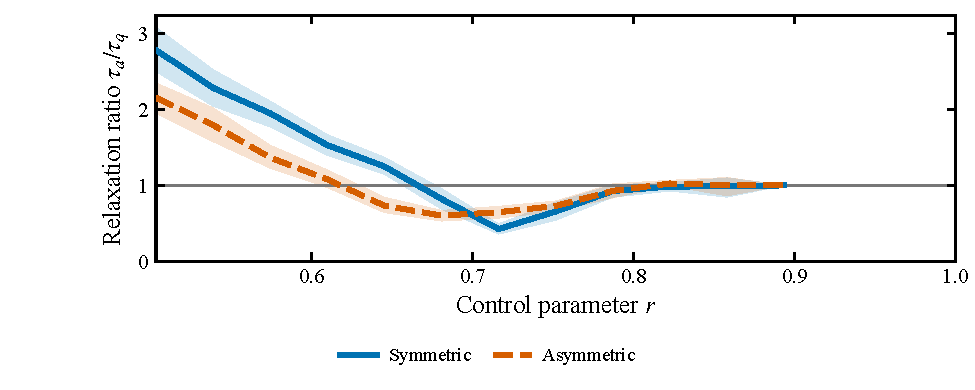
\includegraphics[width=0.92\linewidth]{s2_tau_ratio.pdf}
  \caption{Relaxation-time ratio between activity and polarization. We estimate characteristic relaxation times $\tau_a$ and $\tau_q$ from post-perturbation decay in representative simulations. Under activity-coupled asymmetry, activity typically relaxes faster than polarization ($\tau_a/\tau_q<1$; baseline mean $\approx 0.70$), indicating that activity is not a passive slow variable and motivating joint tracking of $(q,a)$.}
  \label{fig:supp:tau-ratio}
\end{figure}

\subsection{Finite-size diagnostics for locating the transition}
To estimate the transition point in finite sparse networks, we use Binder cumulant crossings because they provide a stable finite-size signature. In contrast, susceptibility peaks can shift non-monotonically with system size and can exhibit pseudo-peaks, making them less reliable for locating $r_c$ in finite simulations.

\begin{figure}[H]
  \centering
  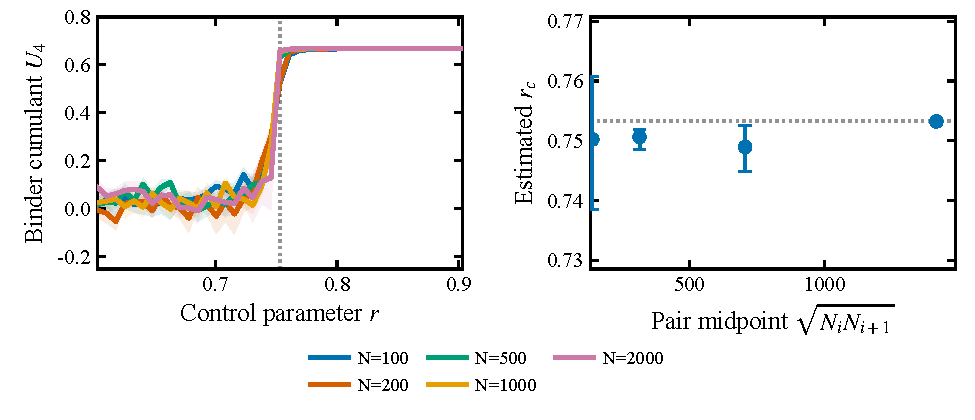
\includegraphics[width=0.92\linewidth]{s2_binder_fss.pdf}
  \caption{Finite-size scaling via Binder cumulant crossings. Binder cumulant curves $U_4(r;N)$ for increasing system sizes cross near the critical region and provide a stable estimator for the effective transition point in finite-$N$ simulations.}
  \label{fig:supp:binder-fss}
\end{figure}

\begin{figure}[H]
  \centering
  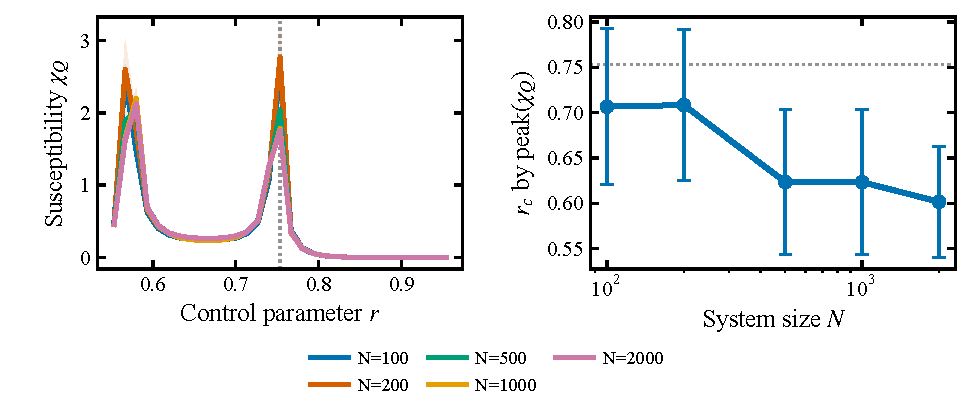
\includegraphics[width=0.92\linewidth]{s2_susceptibility_fss.pdf}
  \caption{Susceptibility-based estimators can be unstable at finite size. Susceptibility peaks may shift non-monotonically with $N$ and can exhibit pseudo-peaks or peak-splitting in finite simulations, motivating the use of Binder crossings as the primary estimator in the main text.}
  \label{fig:supp:susceptibility-fss}
\end{figure}

% -------------------------
% S4: Additional critical-slowing-down diagnostics
% -------------------------
\section{Additional critical-slowing-down diagnostics}
\label{supp:s4-csd}

This note provides additional diagnostics for critical slowing down (CSD) beyond the main-text panels. These analyses emphasize the main narrative point that CSD provides a leading indicator measurable before the transition is crossed.

\subsection{Early-warning statistics across the control parameter}
Approaching the critical point from below, the restoring force weakens and the dynamics become more persistent. This manifests as rising short-lag autocorrelation and variance, which are standard early-warning statistics in the critical-transition literature.

\begin{figure}[H]
  \centering
  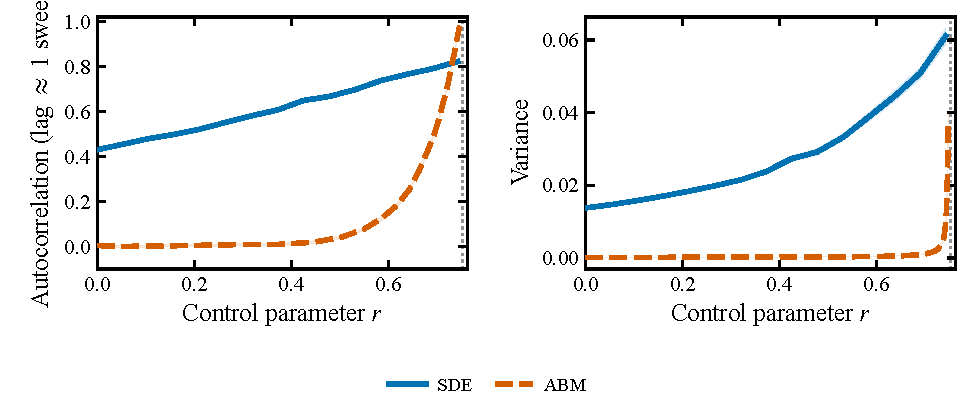
\includegraphics[width=0.92\linewidth]{s3_ews_ac_var.pdf}
  \caption{Early-warning signals from autocorrelation and variance. As $r$ approaches $r_c$ from below, the polarization dynamics exhibit increasing persistence (higher short-lag autocorrelation) and elevated variance, consistent with the weakening restoring force predicted by mean-field theory.}
  \label{fig:supp:ews-ac-var}
\end{figure}

\subsection{Robustness across lag choices}
To confirm that the persistence increase is not an artifact of choosing a particular lag, we compute autocorrelation at multiple lags. The qualitative rise near criticality is consistent across lags.

\begin{figure}[H]
  \centering
  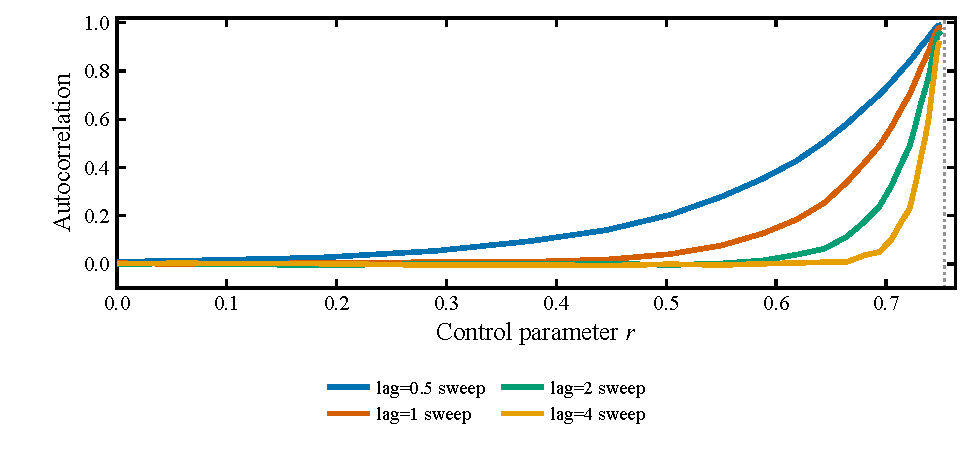
\includegraphics[width=0.92\linewidth]{s3_abm_multilag_ac.pdf}
  \caption{Multi-lag autocorrelation in ABM trajectories. Autocorrelation increases near criticality across multiple lags, supporting the interpretation of rising persistence as a CSD signature rather than a lag-specific plotting choice.}
  \label{fig:supp:abm-multilag-ac}
\end{figure}

% -------------------------
% S5: Additional parameter-landscape analyses
% -------------------------
\section{Additional parameter-landscape analyses}
\label{supp:s5-parameter}

This note provides additional figures supporting the parameter-landscape results in the main text. The goal is to clarify how structural parameters move the critical boundary and to close potential reviewer questions about finite-size artifacts and symmetry assumptions.

\subsection{Symmetry validation}
The analytic critical point is derived in a symmetric validation regime. Along the symmetry constraint, the theoretical constructions satisfy neutrality conditions used in the derivation, supporting the internal consistency of the landscape map.

\begin{figure}[H]
  \centering
  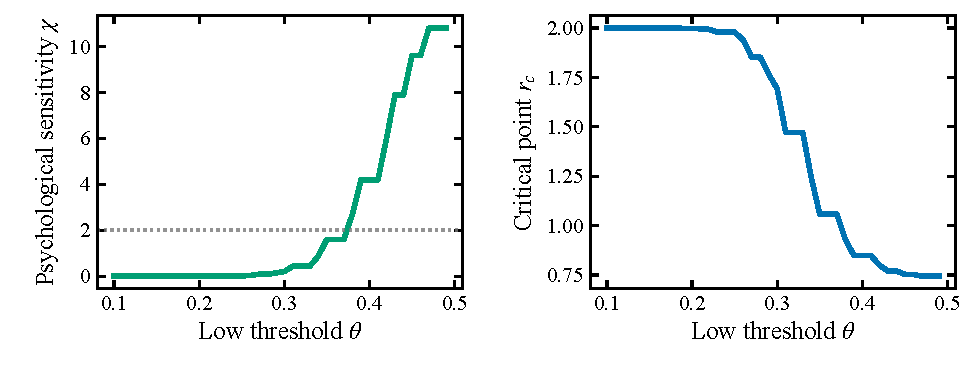
\includegraphics[width=0.92\linewidth]{s4_symmetric_diagonal.pdf}
  \caption{Symmetry diagnostics in the theory-validation regime. Along the symmetric constraint, the theoretical constructions satisfy the expected neutrality conditions used to derive the analytic critical point and the landscape map.}
  \label{fig:supp:symmetric-diagonal}
\end{figure}

\subsection{Decomposing the information-density effect}
The main text reports a non-monotonic $k$ effect on the estimated transition point. We separate this into two components: how $k$ changes the psychological sensitivity $\chi$, and how the induced $\chi(k)$ maps to $r_c(k)$.

\begin{figure}[H]
  \centering
  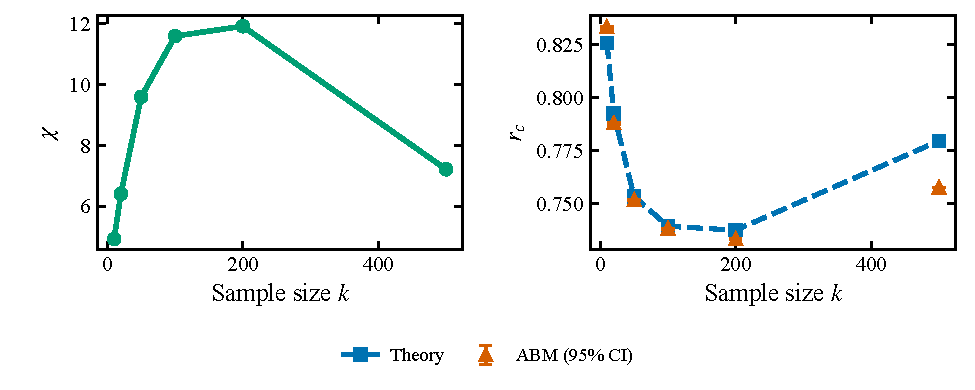
\includegraphics[width=0.92\linewidth]{s4_k_effect_split.pdf}
  \caption{Decomposing the information-density effect. We report additional diagnostics separating how $k$ shapes sensitivity $\chi$ and, through $\chi$, the predicted critical point $r_c$.}
  \label{fig:supp:k-effect-split}
\end{figure}

\subsection{Finite-size closure at high information density}
At very large information density ($k=500$), discrete-threshold effects and finite-size fluctuations can bias naive estimators. Local scanning and finite-size extrapolation reconcile the apparent deviation with the analytic prediction.

\begin{figure}[H]
  \centering
  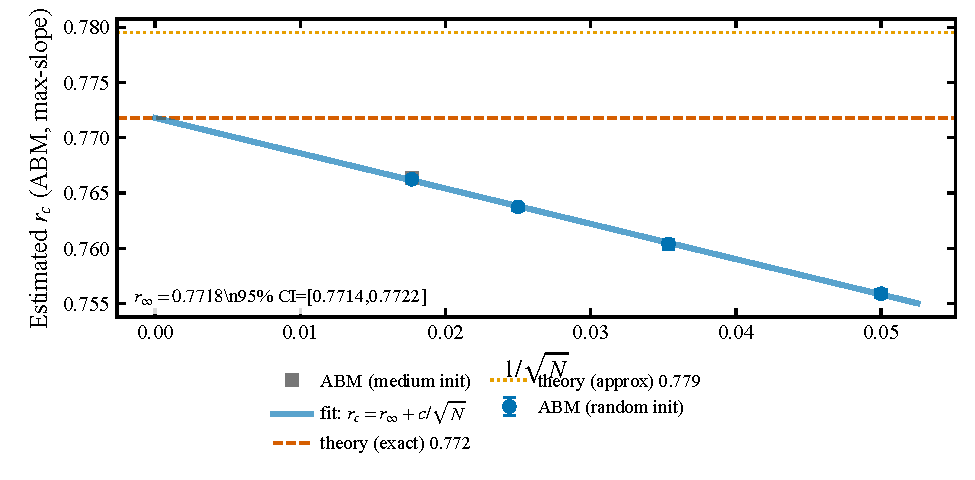
\includegraphics[width=0.92\linewidth]{s4_k500_finite_size.pdf}
  \caption{Finite-size closure for $k=500$. Apparent discrepancies at high information density are resolved by local scanning and finite-size extrapolation, supporting the interpretation that the deviation is a finite-$N$ effect rather than a violation of the analytic prediction.}
  \label{fig:supp:k500-finite-size}
\end{figure}

\subsection{Local coupling and branch-selection bias}
Beyond the well-mixed benchmark, local coupling can introduce reinforcement that both shifts the effective boundary and biases branch selection. These effects help interpret why topology and local interactions matter for proximity to criticality.

\begin{figure}[H]
  \centering
  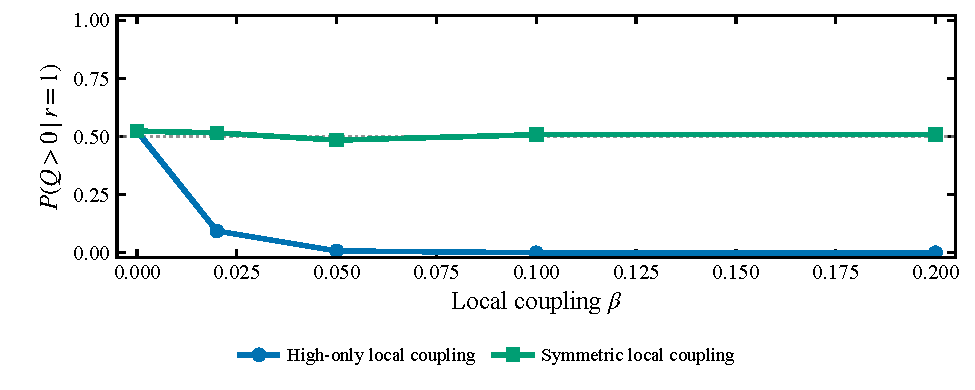
\includegraphics[width=0.92\linewidth]{s4_beta_branch_bias.pdf}
  \caption{Branch-selection bias induced by local coupling. When local coupling $\beta>0$ is introduced, branch selection can become biased, yielding an effective transition behavior that differs from the symmetric well-mixed benchmark.}
  \label{fig:supp:beta-branch-bias}
\end{figure}

\begin{figure}[H]
  \centering
  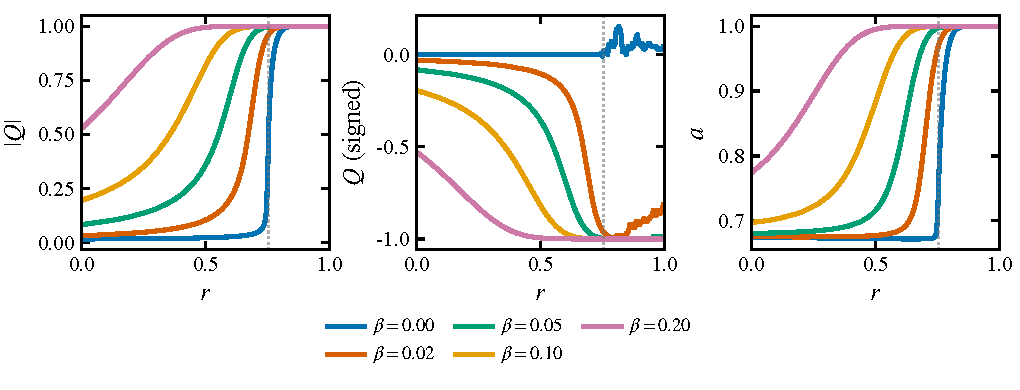
\includegraphics[width=0.92\linewidth]{s4_beta_q_a.pdf}
  \caption{Joint $(q,a)$ effects under local coupling. Local coupling shifts the macroscopic boundary and modifies the relationship between polarization and activity, illustrating how topology and local reinforcement jointly determine proximity to criticality.}
  \label{fig:supp:beta-q-a}
\end{figure}

% -------------------------
% S6: Additional empirical analyses and robustness checks
% -------------------------
\section{Additional empirical analyses and robustness checks}
\label{supp:s6-empirical}

This note provides additional empirical figures supporting the main-text empirical section. The main narrative purpose is to make explicit the empirical constraints---non-uniform sampling density and missing windows---and to show that the two empirical signatures are assessed with diagnostics aligned to the theory: activity as a precursor of jump intensity and media composition as a driver of volatility.

\noindent\textbf{Dataset convention.} For compact visualization, we label the three empirical subsets as Dataset A (official-media topic set), Dataset B (high-density discussion set used for the primary empirical tests), and Dataset C (their merged sample). These labels are used only in Supplementary figures.

\subsection{Time-series overview and segmentation rationale}
We first summarize the window-level proxies used in the main text and highlight missingness patterns. This motivates segment-based aggregation and density-aware diagnostics used in subsequent panels.

\begin{figure}[H]
  \centering
  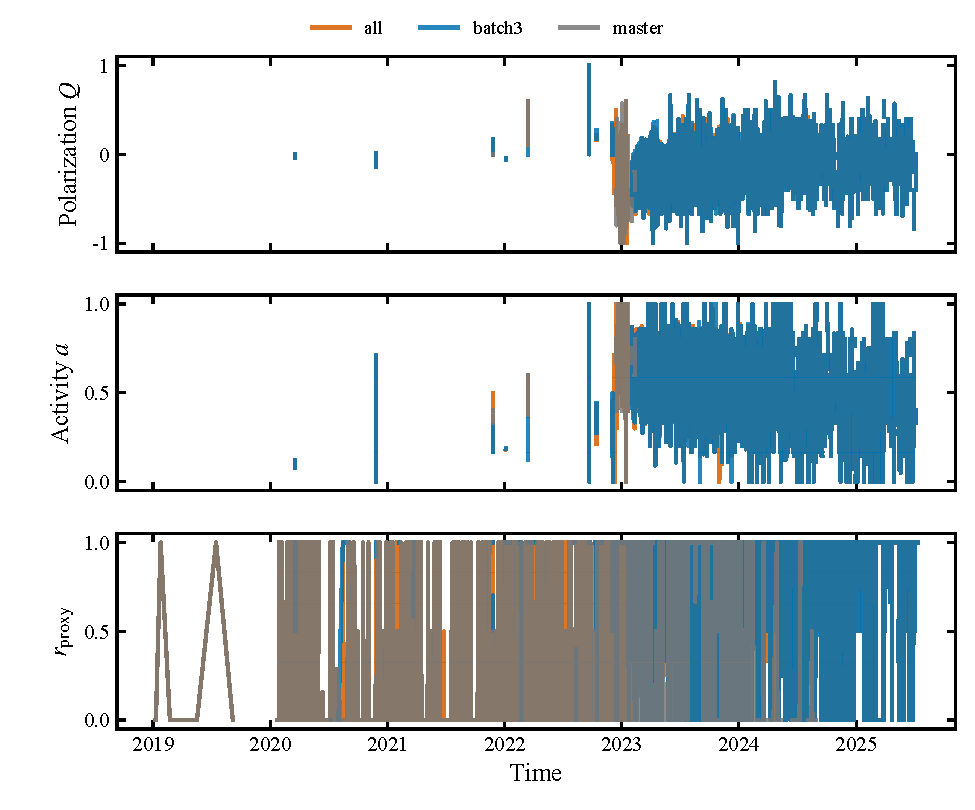
\includegraphics[width=0.92\linewidth]{s5_time_series_overview.pdf}
  \caption{Time-series overview across datasets (Dataset A/B/C as defined above). We show the 4-hour aggregates used to compute window-level proxies $(Q,a,r_{\text{proxy}})$, highlighting the non-uniform sampling density and the resulting need for segment-based aggregation in the main-text analyses.}
  \label{fig:supp:time-series-overview}
\end{figure}

\subsection{Scatter diagnostics for the two empirical signatures}
To connect directly to the theoretical mechanism, we evaluate two segment-level associations under the primary 4-hour aggregation: elevated activity predicting larger polarization jumps, and increased user-generated dominance predicting higher polarization volatility. Density stratification is shown to diagnose coverage-driven confounds. The main text reports the density-controlled H2 estimate under 12-hour aggregation; the 4-hour diagnostics here provide additional context across datasets and missingness patterns.

\begin{figure}[H]
  \centering
  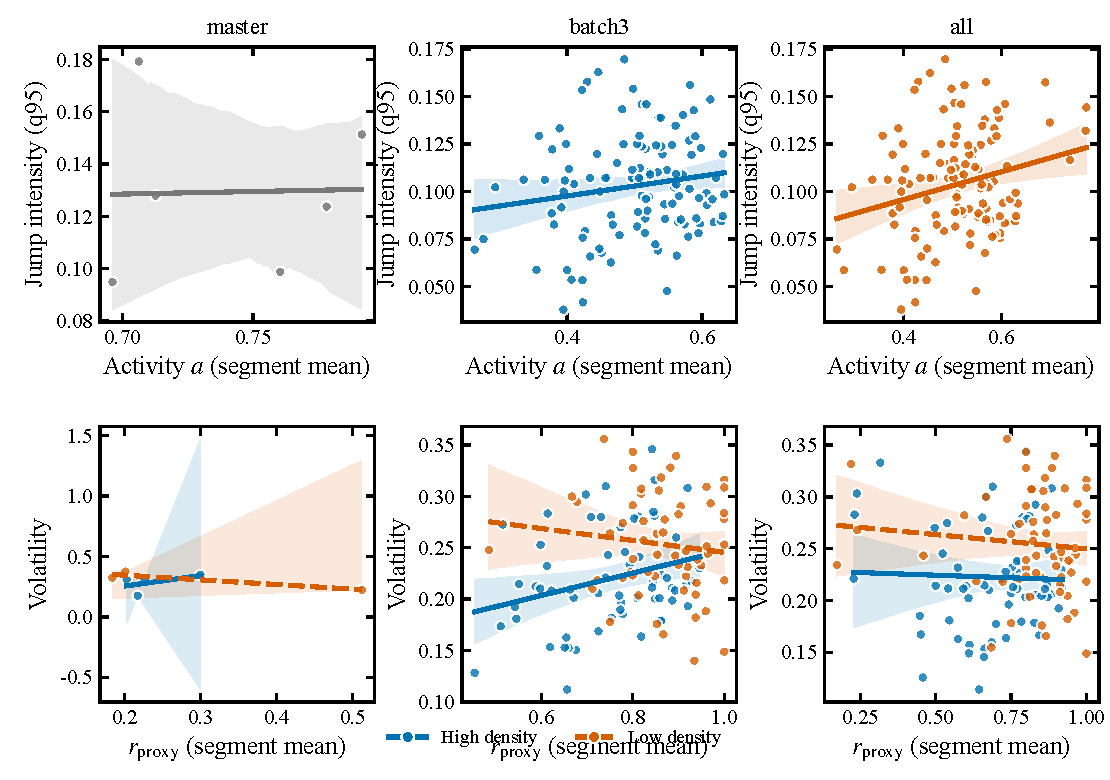
\includegraphics[width=0.92\linewidth]{s5_scatter_h1_h2.pdf}
  \caption{Scatter diagnostics for empirical signatures under the primary 4-hour aggregation across datasets (Dataset A/B/C as defined above). We show the segment-level associations for the activity--jump and media-dominance--volatility tests, including density-stratified views used to diagnose sampling-coverage confounds.}
  \label{fig:supp:scatter-h1-h2}
\end{figure}

\subsection{Event-aligned early-warning analysis under realistic missingness}
We additionally assess early-warning behavior by aligning autocorrelation/variance indicators to jump events. Continuity requirements can make high-frequency aggregation infeasible in sparse datasets, which limits the strength of event-aligned tests.

\begin{figure}[H]
  \centering
  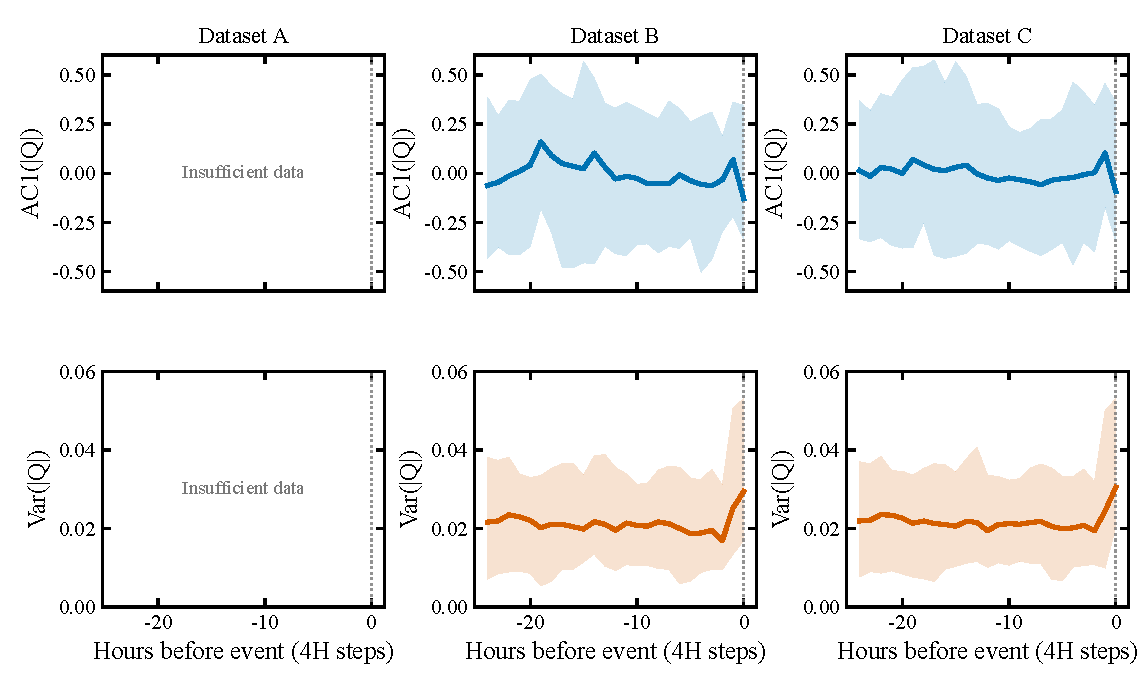
\includegraphics[width=0.92\linewidth]{s5_eventstudy_h4.pdf}
  \caption{Additional details for event-aligned early-warning analysis (Dataset A/B/C as defined above). We report event-aligned trajectories for autocorrelation and variance indicators under the primary 4-hour aggregation and illustrate how higher-frequency aggregation (e.g., 2H/1H) can become infeasible due to continuity requirements, motivating the limitations statement in the main text.}
  \label{fig:supp:eventstudy-h4}
\end{figure}

\subsection{Density-controlled H2 under 12H aggregation}
We report the media-dominance--volatility association under 12-hour aggregation, which increases per-window sample size at the cost of temporal granularity and stabilizes within-segment estimates of $r_{\text{proxy}}$ and volatility. The positive association remains significant after controlling for segment sampling density, supporting that the media-ecology signature is not explained by coverage alone.

\begin{figure}[H]
  \centering
  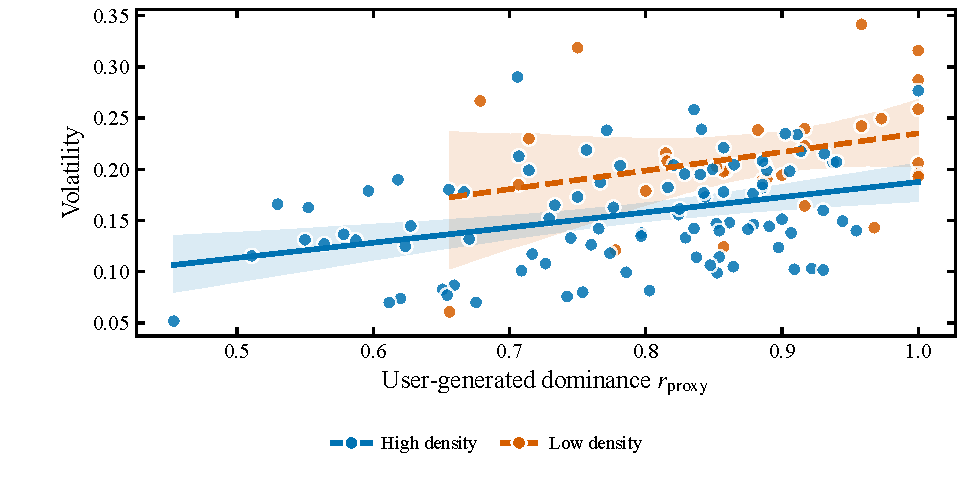
\includegraphics[width=0.92\linewidth]{s5_h2_density_12h.pdf}
  \caption{Density-controlled media-dominance--volatility signature under 12-hour aggregation. The analysis yields a positive association between $r_{\text{proxy}}$ and volatility (Pearson $r=0.429$, $p=6.03\times 10^{-7}$; partial $r=0.386$, $p=8.79\times 10^{-6}$ controlling for the number of valid windows per week; median split at 14 windows). Solid/dashed lines show groupwise linear fits with 95\% bootstrap bands.}
  \label{fig:supp:h2-density-12h}
\end{figure}

% Add additional supplementary notes, figures, and tables below.

\FloatBarrier
\bibliographystyle{unsrt}
\bibliography{references}
\end{document}
